\section{Руководство пользователя}
\label{sec:user_guide}

\subsection{Управление аккаунтом} 
\label{sec:user_guide:account}

При входе на сайт первое, что должен сделать пользователь, это зарегистрироваться в системе.
Только зарегистрированные пользователи могут приобретать игры и оставлять отзывы. Для создания нового аккаунта необходимо выбрать пункт
"Вход"\ на панели навигации, и на появившейся странице нажать на кнопку "Нет аккаунта?". После этого пользователь будет перенаправлен
на форму регистрации (Рисунок \ref*{sec:user_guide:account:register}), где необходимо ввести адрес электронной почты и придумать пароль.
После успешной регистрации пользователь будет перенаправлен к форме входа и сможет войти в созданный аккаунт.

Авторизованному пользователю становятся доступен основной функционал сайта и отображаются новые пункты в навигационной панели. Среди
них есть пункт "Аккаунт", при переходе к которому пользователь может сменить свой пароль, заполнив соответствующую форму (Рисунок \ref*{sec:user_guide:account:passwordchange}).

Также, в случае если пользователь забыл свой пароль и не может войти в аккаунт, он имеет возможность восстановить доступ. Для этого
на странице входа необходимо нажать на кнопку "Забыли пароль?"\ , после чего пользователь будет перенаправлен на соответствующую страницу
(Рисунок \ref*{sec:user_guide:account:restore}). Для восстановления доступа необходимо ввести почту, к которой привязан аккаунт, и 
нажать на кнопку "Отправить" справа от поля. После этого на указанный почтовый ящик пользователю придёт письмо с кодом для восстановления,
который необходимо ввести в поле "Пароль" и нажать на кнопку "Отправить" внизу формы. Пользователь будет авторизован в системе и перенаправлен
на страницу для смены пароля.

\begin{figure}[ht]
	\centering
	  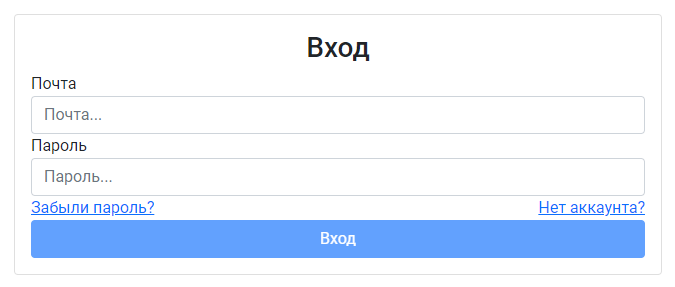
\includegraphics[scale=0.8]{attachments/register.png}  
	  \caption{ Форма для регистрации }
	  \label{sec:user_guide:account:register}
\end{figure}

\begin{figure}[ht]
	\centering
	  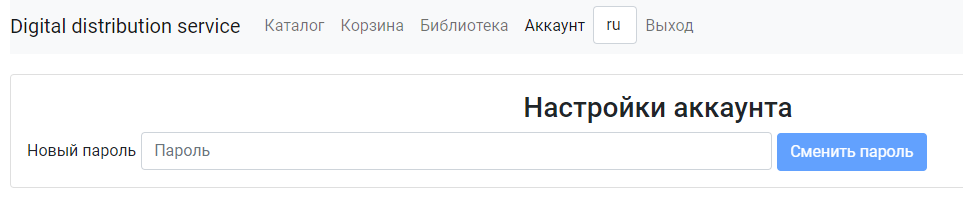
\includegraphics[scale=0.55]{attachments/passwordchange.png}  
	  \caption{ Форма для смены пароля }
	  \label{sec:user_guide:account:passwordchange}
\end{figure}

\begin{figure}[ht]
	\centering
	  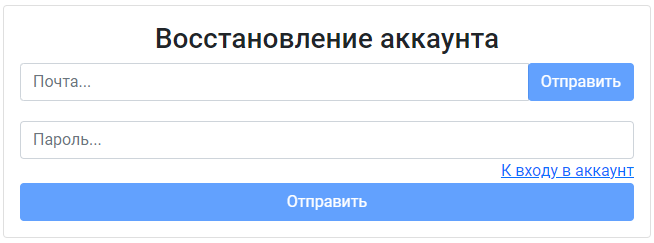
\includegraphics[scale=0.8]{attachments/restore.png}  
	  \caption{ Форма для восстановления доступа к аккаунту }
	  \label{sec:user_guide:account:restore}
\end{figure}

\subsection{Основной функционал} 
\label{sec:user_guide:main}

После того, как пользователь вошёл в свой аккаунт, ему становится доступен основной функционал сервиса, который включает в себя
добавление игр в корзину, приобретение видеоигр и написание обзоров. На панели навигации появляются пункты "Корзина"\ и "Библиотека".
Для добавления игр в корзину необходимо нажать на соответствующую кнопку в каталоге напротив выбранной игры. После этого кнопка становится
неактивной, а игра помещается в корзину пользователя. Количество игр в корзине не ограничено. Когда пользователь определился с выбором и
хочет приобрести игры, он должен перейти в корзину через пункт на панели навигации (Рисунок \ref*{sec:user_guide:main:cart}). Там он 
может ознакомиться со списком игр готовых к приобритению, увидеть суммарную стоимость и по желанию удалить продукты из корзины. После
нажатия на кнопку "Оплатить"\ , игры будут помещены в библиотеку пользователя, попасть в которую можно выбрав соответствующий пункт на панели
навигации (Рисунок \ref*{sec:user_guide:main:library}). Для того, чтобы оставить отзыв, необходимо нажать на кнопку "Обновить обзор"\
напротив выбранной игры, и заполнить появившуюся форму. Там же можно отредактировать уже существующий обзор либо удалить его. Все пользовательские
обзоры видны в каталоге игр -- напротив игры появляется её средняя оценка и ссылка на все обзоры. По нажатию на эту ссылку пользователь
попадает на страницу обзоров, где может подробнее ознакомиться с ними (Рисунок \ref*{sec:user_guide:main:reviews}).

\begin{figure}[ht]
	\centering
	  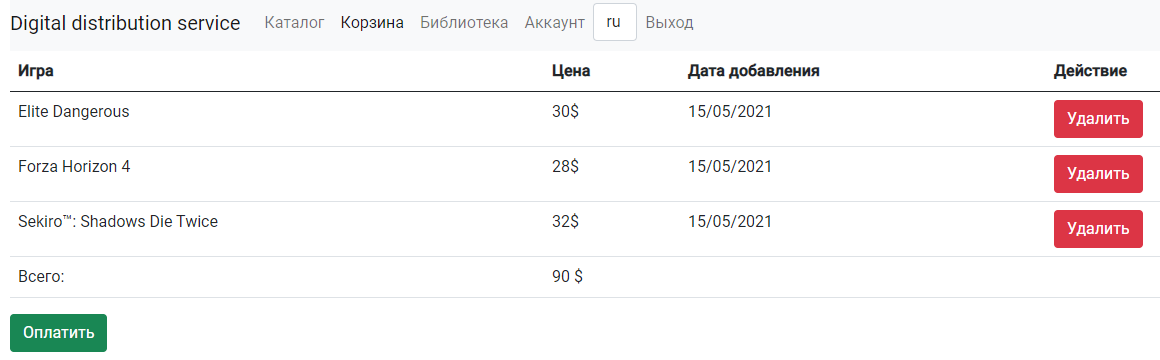
\includegraphics[scale=0.4]{attachments/cart.png}  
	  \caption{ Корзина пользователя }
	  \label{sec:user_guide:main:cart}
\end{figure}

\begin{figure}[ht]
	\centering
	  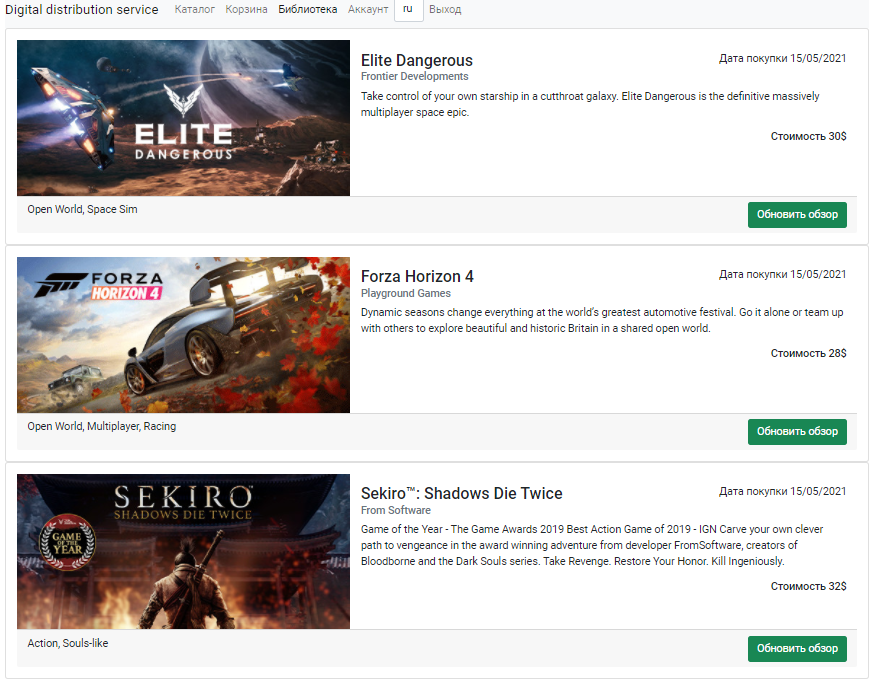
\includegraphics[scale=0.4]{attachments/library.png}  
	  \caption{ Библиотека пользователя }
	  \label{sec:user_guide:main:library}
\end{figure}

\begin{figure}[!htb]
	\centering
	  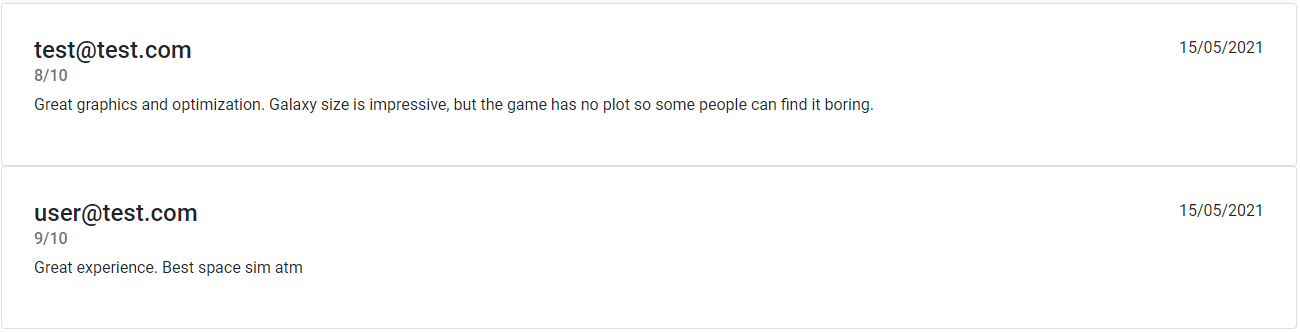
\includegraphics[scale=0.4]{attachments/reviews.png}  
	  \caption{ Подробный просмотр обзоров }
	  \label{sec:user_guide:main:reviews}
\end{figure}

\subsection{Функционал администратора} 
\label{sec:user_guide:admin}

Пользователь с ролью "Администратор" обладает дополнительными возможностями в сервисе. Для того, чтобы добавить аккаунт администратора,
необходимо создать запись о новом пользователе с соответствующей ролью в базе данных. При входе в аккаунт администратора, на панели
навигации появляется новый пункт "Админ"\ , по нажатию на который пользователь попадает на панель администратора. Отсюда он может управлять
жанрами и добавлять в каталог новые игры. По нажатию на кнопку "Управление жанрами"\ , пользователь будет перенаправлен на страницу, где
можно просмотреть список всех жанров в системе, удалить выбранные, либо добавить новые (Рисунок \ref*{sec:user_guide:admin:genres}).
По нажатию на кнопку "Добавить игру"\ , администратор попадает на страницу для добавления новой игры в каталог (Рисунок \ref*{sec:user_guide:admin:addgame}).
Для этого необходимо выбрать изображение и заполнить все поля формы. Справа от формы можно добавить к игре несколько жанров из присутствующих
в системе.

Дополнительный функционал также появляется на странице с каталогом игр. Здесь напротив каждой игры возникают две дополнительные кнопки:
"Удалить"\ и "Изменить"\ , нажав на которые администратор может удалить игру из каталога либо отредактировать её описание и жанры (Рисунок \ref*{sec:user_guide:admin:catalog}).

\begin{figure}[ht]
	\centering
	  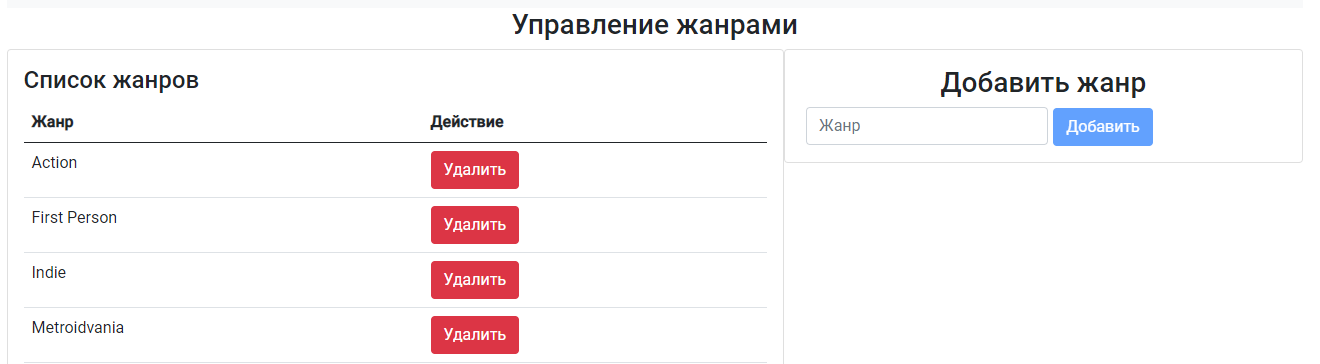
\includegraphics[scale=0.4]{attachments/genres.png}  
	  \caption{ Управление жанрами }
	  \label{sec:user_guide:admin:genres}
\end{figure}

\begin{figure}[ht]
	\centering
	  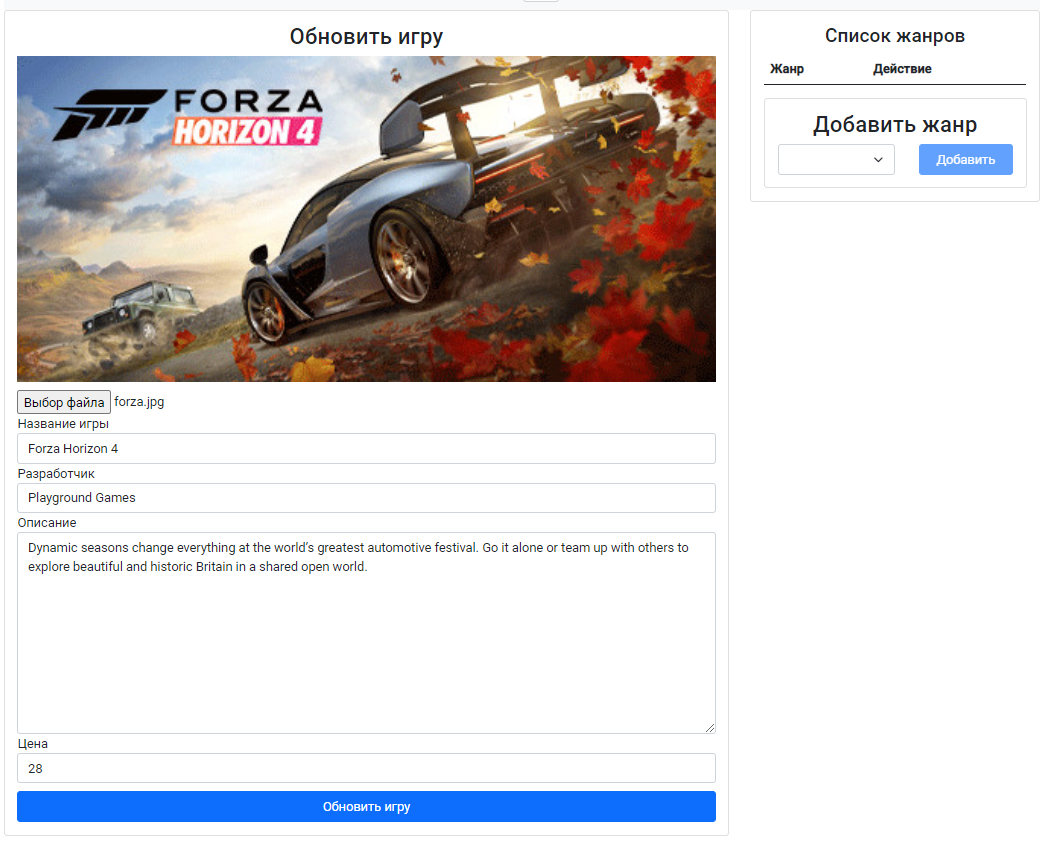
\includegraphics[scale=0.32]{attachments/addgame.png}  
	  \caption{ Добавление игры }
	  \label{sec:user_guide:admin:addgame}
\end{figure}
\clearpage
\begin{figure}[!ht]
	\centering
	  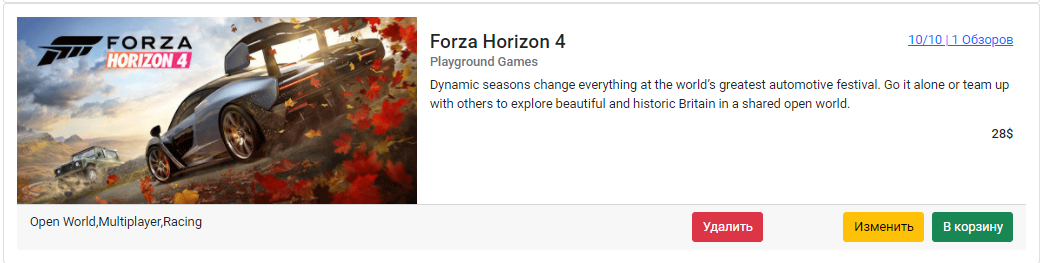
\includegraphics[scale=0.4]{attachments/catalog.png}  
	  \caption{ Дополнительный функционал в каталоге }
	  \label{sec:user_guide:admin:catalog}
\end{figure}
